%% ============================================================================
%%  Hardware-light neural response estimation for naturalistic video
%%  A Methods manuscript prepared for the Frontiers in Computational Neuroscience
%%  Research Topic: "Digital phenotyping and neuro-simulations: Scaling
%%  precision neuroscience via IT" (manuscript deadline 19 Nov 2026).
%%
%%  PORTING TO THE OFFICIAL FRONTIERS TEMPLATE
%%  ------------------------------------------
%%  This file compiles standalone with the standard `article` class so it can
%%  be read and reviewed anywhere (pdflatex main.tex; bibtex main; pdflatex x2).
%%  To submit, download the Frontiers LaTeX template (frontiersinSCNS.cls,
%%  Computational Neuroscience) and paste the body sections below into it. The
%%  section order and names here match the Frontiers Methods layout 1:1.
%%
%%  INTEGRITY NOTE (do not remove): every empirical statement below reflects
%%  what the committed notebooks actually executed. The runs used STOCK
%%  pretrained TRIBE v2 (no custom weights), were BIMODAL (video+audio; the
%%  text/language pathway was inactive), and the prediction arrays were not
%%  persisted, so no quantitative neural results are claimed. See Section 2.5.
%% ============================================================================
\documentclass[11pt]{article}

\usepackage[utf8]{inputenc}
\usepackage[T1]{fontenc}
\usepackage{lmodern}
\usepackage[htt]{hyphenat} % allow long \texttt tokens (hashes, code) to wrap
\usepackage[margin=1in]{geometry}
\usepackage{graphicx}
\usepackage{booktabs}
\usepackage{amsmath}
\usepackage{amssymb}
\usepackage{siunitx}
\usepackage{xcolor}
\usepackage{tikz}
\usetikzlibrary{arrows.meta, positioning, fit, backgrounds}
\usepackage[hidelinks]{hyperref}
\usepackage[numbers,sort&compress]{natbib}
\usepackage{authblk}
\usepackage{caption}
\usepackage{enumitem}

\captionsetup{font=small,labelfont=bf}
\setlength{\parskip}{0.35em}
\renewcommand{\arraystretch}{1.15}

% --- Title ------------------------------------------------------------------
\title{\vspace{-2em}\bfseries Hardware-light neural response estimation for
naturalistic video: a reproducible protocol using an open multimodal
brain-encoding foundation model}

% Authors: Ruhani Gill (student author), supervised by Dr Misha Kakkar.
% The four Research Topic editors (S.\ Khan, D.\ Mehrotra, S.\ Bhartiya,
% A.\ Garg) are EDITORS, not co-authors, and must NOT appear here.
\author[1]{Ruhani Gill}
\author[1,*]{Misha Kakkar}
\affil[1]{Amity University, Noida, Uttar Pradesh, India}
\affil[*]{Correspondence: \texttt{mkakkar@amity.edu}}

\date{}

\begin{document}
\maketitle

% ============================================================================
\begin{abstract}
\noindent
Traditional neuromarketing and, more broadly, stimulus--response neuroscience
rely on electroencephalography (EEG) or functional magnetic resonance imaging
(fMRI), which are costly, slow, and hard to scale beyond a handful of
participants. Recent multimodal \emph{brain-encoding foundation models} predict
cortical responses to naturalistic audio--visual stimuli directly from the
stimulus, offering a ``hardware-light, software-heavy'' alternative that
requires no scanner and no participant at inference time. We present a
\emph{reproducible protocol} that operationalises one such model---the
open-source TRIBE~v2 trimodal brain encoder---for estimating vertex-wise
cortical activity from short naturalistic video, using free cloud computation
(Google Colab, one T4 GPU). We document the full pipeline: video ingestion,
automatic speech transcription, per-modality feature extraction, and
projection onto the \texttt{fsaverage5} cortical surface (20{,}484 vertices) at
a one-second sampling interval. As a feasibility demonstration we first
reproduce the model's documented reference behaviour on a standard trailer
clip, then apply the protocol to three fast-moving-consumer-goods (FMCG)
television advertisements. We report the pipeline's compute characteristics and
qualitative output, and we are explicit about the demonstration's boundaries:
the runs were bimodal (video and audio; the language pathway was inactive), the
predicted activity arrays were not persisted, and no ground-truth neural data
were available, so we make no quantitative accuracy claim. To close that gap we
specify a pre-registered validation protocol---self-report affect ratings and
public engagement metrics correlated against persisted per-region
predictions---together with a power analysis. The contribution is a
transparent, transferable method and an open, auditable recipe for
scanner-free neural response estimation, applicable well beyond advertising to
clinical naturalistic-stimulus paradigms.

\vspace{0.6em}
\noindent\textbf{Keywords:} brain encoding, foundation models, neuro-simulation,
naturalistic stimuli, digital phenotyping, reproducibility, explainable AI,
open science
\end{abstract}

% ============================================================================
\section{Introduction}

Understanding how the human brain responds to rich, naturalistic stimuli is a
central goal of both cognitive neuroscience and its applied offshoots. In
consumer neuroscience---``neuromarketing''---the question is narrower but
concrete: which moments of an advertisement engage a viewer, and how strongly
\citep{ariely2010,plassmann2015}. The dominant measurement tools, EEG and fMRI,
are powerful but expensive, slow, and difficult to scale: a single fMRI session
can cost hundreds to thousands of units of currency, recruitment and scheduling
take weeks, and sample sizes rarely exceed a few dozen participants
\citep{poldrack2017}. These constraints are not unique to marketing; they limit
any programme that seeks to characterise brain responses to many stimuli, many
times, at low marginal cost---precisely the regime that ``precision
neuroscience at scale'' demands.

A complementary strategy has matured rapidly: rather than \emph{measuring} the
brain for every new stimulus, one can \emph{predict} its response with an
\emph{encoding model} learned from prior recordings
\citep{naselaris2011,huth2016}. Classical encoding models map hand-designed or
network-derived stimulus features onto voxel- or vertex-wise activity. The
current generation replaces bespoke features with large pretrained
representations and couples them to the cortical surface through a shared
transformer, yielding \emph{brain-encoding foundation models} that generalise
across stimuli and, to a degree, across people. TRIBE~v2 (Trimodal Brain
Encoder) is a recent open example: it fuses video, audio, and text
representations---from V-JEPA\,2 / DINOv2, Wav2Vec-BERT, and Llama~3.2
respectively---and predicts fMRI activity across the whole cortical surface for
naturalistic movie stimuli \citep{tribe2025,vjepa2,dinov2,wav2vecbert,llama3}.
Because inference needs only the stimulus and a GPU, such models turn a
hardware problem into a software one.

This ``hardware-light, software-heavy'' shift is exactly the opening that the
present Research Topic identifies: automated, secure, scalable tools for brain
monitoring and analysis, built from open software pipelines rather than new
instrumentation. Our aim here is deliberately methodological. We do \emph{not}
claim a new model, and we do \emph{not} claim validated neuromarketing findings.
Instead we contribute:

\begin{enumerate}[leftmargin=1.4em,itemsep=0.15em,topsep=0.25em]
  \item A \textbf{reproducible, low-cost protocol} for estimating vertex-wise
  cortical responses to short naturalistic videos using an open brain-encoding
  foundation model on free cloud hardware, specified precisely enough to
  re-run (exact package pins, model snapshot, and step-by-step procedure;
  Section~\ref{sec:methods}).
  \item A \textbf{transparent feasibility demonstration} on three FMCG
  advertisements, benchmarked against the model's documented reference
  behaviour, with an honest account of what the runs did and did not establish
  (Section~\ref{sec:results}).
  \item A \textbf{pre-specified validation protocol}---self-report affect and
  public engagement metrics against persisted per-region predictions, with a
  power analysis---that any group can execute to convert the demonstration into
  a quantitative study (Section~\ref{sec:validation}).
\end{enumerate}

We frame advertising merely as a convenient, license-clear stimulus domain.
The same protocol applies to any naturalistic-video paradigm, including the
clinical assessment settings---using film as a standardised cognitive
probe---that motivate this Research Topic (Section~\ref{sec:discussion}).

% ============================================================================
\section{Materials and Methods}
\label{sec:methods}

The protocol takes a short video file and returns a matrix of predicted
cortical activity of shape $T \times V$, where $T$ is the number of
one-second time steps (TRs) and $V=20{,}484$ is the number of vertices on the
\texttt{fsaverage5} surface. Figure~\ref{fig:pipeline} summarises the flow.

% --- Pipeline schematic (inline TikZ, no external asset) --------------------
\begin{figure}[t]
\centering
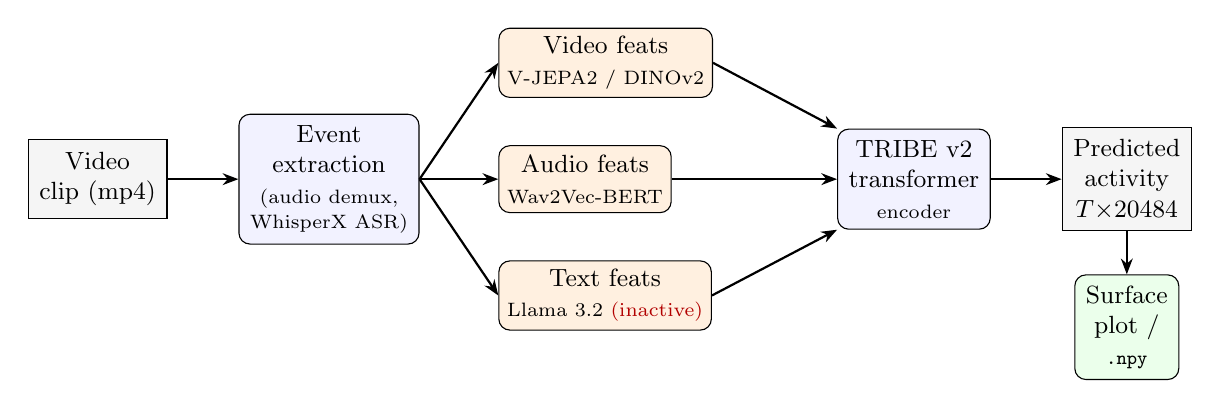
\begin{tikzpicture}[
  font=\small,
  node distance=0.55cm and 0.9cm,
  box/.style={draw, rounded corners, align=center, minimum height=1.0cm,
              inner sep=4pt, fill=blue!5},
  mod/.style={draw, rounded corners, align=center, minimum height=0.85cm,
              inner sep=3pt, fill=orange!12},
  io/.style={draw, align=center, minimum height=1.0cm, inner sep=4pt,
             fill=gray!8},
  arr/.style={-{Stealth[length=2mm]}, thick}
]
\node[io] (vid) {Video\\ clip (mp4)};
\node[box, right=of vid] (ev) {Event\\ extraction\\ \scriptsize (audio demux,\\[-2pt]
  \scriptsize WhisperX ASR)};
\node[mod, above right=0.2cm and 1.0cm of ev] (v) {Video feats\\ \scriptsize V-JEPA2 / DINOv2};
\node[mod, right=1.0cm of ev] (a) {Audio feats\\ \scriptsize Wav2Vec-BERT};
\node[mod, below right=0.2cm and 1.0cm of ev] (t) {Text feats\\ \scriptsize Llama 3.2
  \textcolor{red!70!black}{\scriptsize (inactive)}};
\node[box, right=2.1cm of a] (tr) {TRIBE~v2\\ transformer\\ \scriptsize encoder};
\node[io, right=of tr] (out) {Predicted\\ activity\\ $T{\times}20484$};
\node[box, below=0.55cm of out, fill=green!8] (viz) {Surface\\ plot /\\ \scriptsize \texttt{.npy}};

\draw[arr] (vid) -- (ev);
\draw[arr] (ev.east) -- (v.west);
\draw[arr] (ev.east) -- (a.west);
\draw[arr] (ev.east) -- (t.west);
\draw[arr] (v.east) -- (tr.north west);
\draw[arr] (a.east) -- (tr.west);
\draw[arr] (t.east) -- (tr.south west);
\draw[arr] (tr) -- (out);
\draw[arr] (out) -- (viz);
\end{tikzpicture}
\caption{\textbf{Protocol overview.} A video clip is decomposed into
time-stamped events; per-modality encoders produce feature streams that the
TRIBE~v2 transformer maps onto the \texttt{fsaverage5} cortical surface at
1\,s resolution. In the demonstration runs the text/language pathway (dashed,
red) was inactive because word-level events were filtered out before
prediction (Section~\ref{sec:deviation}). The predicted-activity matrix should
be persisted (\texttt{.npy}) to enable quantitative analysis; in the present
runs only the rendered surface plots survive.}
\label{fig:pipeline}
\end{figure}

\subsection{Model}
We use \textbf{TRIBE~v2}, an open multimodal brain-encoding model distributed
through the Hugging Face Hub as \texttt{facebook/tribev2}
\citep{tribe2025}. The model was loaded from checkpoint \texttt{best.ckpt}
(\SI{709}{\mega\byte}; snapshot
\texttt{f894e783020944dcd96e5568550afe2aa9743f9f}) via the project's
\texttt{TribeModel.from\_pretrained} utility, with no modification to weights or
architecture. TRIBE~v2 ingests three modalities through pretrained encoders---
video via V-JEPA\,2 and DINOv2, audio via Wav2Vec-BERT, and text via
Llama~3.2 \citep{vjepa2,dinov2,wav2vecbert,llama3}---and predicts blood-oxygen-
level-dependent (BOLD) activity for each of $V=20{,}484$ vertices of the
\texttt{fsaverage5} template surface \citep{fischl2012} at a repetition time of
$\mathrm{TR}=\SI{1}{\second}$. Following the model's convention, predictions are
aligned to the stimulus with a \SI{5}{\second} offset to compensate for the
hemodynamic lag. Speech is transcribed to word-level events with WhisperX
\citep{whisperx,radford2023}.

\subsection{Compute environment and reproducibility}
\label{sec:repro}
All runs were performed on Google Colab with a single NVIDIA T4 GPU. The
software environment is pinned as follows (harvested from the executed notebook
logs), which we report so the runs can be reproduced exactly:

\begin{itemize}[leftmargin=1.4em,itemsep=0.1em,topsep=0.2em]
  \item \texttt{tribev2==0.1.0} installed from source at commit\\
        {\footnotesize\texttt{af58661791a351a448a489042a28f6c37e1c14b7}};
  \item \texttt{torch==2.6.0}, \texttt{torchvision==0.21.0},
        \texttt{torchaudio==2.6.0} (force-reinstalled to match), with the
        CUDA~12.4 runtime stack;
  \item \texttt{x-transformers==1.27.20}, \texttt{triton==3.2.0},
        \texttt{torchmetrics==1.9.0}, \texttt{submitit==1.5.4};
  \item plotting stack \texttt{pyvista==0.48.4}, \texttt{vtk==9.6.2}.
\end{itemize}

\noindent The install pins \texttt{pandas==3.0.3}, which is newer than some
preinstalled Colab packages expect (\texttt{cudf}, \texttt{dask-cudf},
\texttt{gcsfs} emit dependency warnings); these warnings did not affect the
pipeline. The install command was
{\footnotesize
\begin{verbatim}
uv pip install \
    "tribev2[plotting] @ git+https://github.com/facebookresearch/tribev2.git"
pip install torchaudio==2.6.0 --force-reinstall --quiet
\end{verbatim}
}
Two GPU-resident feature encoders dominate memory: the audio encoder
(\SI{2.32}{\giga\byte}) and the video encoder (\SI{4.14}{\giga\byte}).

\subsection{Stimulus set}
\label{sec:stimuli}
The demonstration uses three publicly broadcast Indian FMCG television
advertisements, chosen to span product categories and audio styles
(Table~\ref{tab:runs}): a Lay's potato-chips spot (``More smiles per mile''), a
Colgate Visible White toothpaste spot (Hindi voice-over), and a Surf Excel
detergent spot (``Primary Colours''). Each was downloaded at 360p and supplied
to the pipeline as an \texttt{mp4}. As a methodological control we also
reproduce the model's documented reference run on the Sintel open-movie trailer
\citep{sintel}. We use advertising because such clips are short, richly
multimodal, and freely available; no human participants were recruited or
recorded, so the demonstration carries no personal neural data
(Section~\ref{sec:ethics}).

\subsection{Procedure}
\label{sec:procedure}
For each clip the protocol executes five steps:
\begin{enumerate}[leftmargin=1.5em,itemsep=0.12em,topsep=0.2em]
  \item \textbf{Ingest.} Load the \texttt{mp4}; the toolkit demultiplexes the
  audio track to \texttt{wav}.
  \item \textbf{Build events.} \texttt{model.get\_events\_dataframe(video\_path)}
  produces a time-stamped event table containing \texttt{Video} and
  \texttt{Audio} spans plus WhisperX-derived \texttt{Word}/\texttt{Sentence}/
  \texttt{Text} events.
  \item \textbf{Select events.} The demonstration retained only
  \texttt{Video} and \texttt{Audio} events\\
  {\footnotesize\texttt{df[df['type'].isin(['Video','Audio'])]}}; see
  Section~\ref{sec:deviation}.
  \item \textbf{Predict.} \texttt{preds, segments = model.predict(events=df)}
  returns activity of shape $T \times 20484$ and the corresponding time
  segments.
  \item \textbf{Visualise.} \texttt{PlotBrain(mesh="fsaverage5")} renders the
  first 15 TRs on the lateral cortical surface (\texttt{cmap="fire"},
  \texttt{norm\_percentile=99}), with the stimulus frame shown above each panel.
\end{enumerate}

\subsection{A documented deviation, and the fix}
\label{sec:deviation}
Two properties of the demonstration runs must be stated plainly because they
bound every downstream interpretation.

\textbf{(i) The runs were bimodal, not trimodal.} Step~3 above removed all
word-level events, so no \texttt{Text} events reached the model and the
Llama~3.2 language pathway was inactive. This is directly visible in the
figures: the ``Text'' track is empty for all three advertisements
(Figure~\ref{fig:ads}) whereas it is populated for the trimodal reference run
(Figure~\ref{fig:reference}, words appearing at $t=12$--$14\,\mathrm{s}$). For
advertisements built around a spoken message---particularly the Hindi-language
Colgate spot---suppressing the language pathway is a material limitation, not a
detail. We report it as such and do not interpret any language-network
activity.

\textbf{(ii) The predicted arrays were not persisted.} The runs rendered the
surface plots but did not save \texttt{preds} to disk. Because the plots are
percentile-thresholded, alpha-composited colour renders, the underlying
$T\times20484$ values cannot be recovered from them. Consequently \emph{no}
quantitative neural result (region-of-interest time courses, cross-ad
comparisons, an ``engagement index'') can be computed from the existing
outputs. The remedy is a single line after Step~4---
{\footnotesize
\begin{verbatim}
import numpy as np; np.save("preds.npy", preds)
\end{verbatim}
}
---which we adopt as a mandatory step of the protocol going forward. Every
quantitative analysis in Section~\ref{sec:validation} presupposes it.

% ============================================================================
\section{Validation protocol (pre-specified)}
\label{sec:validation}

Because the present runs yield no persisted predictions, we specify---rather
than report---a validation study. Stating it in advance makes the eventual
analysis falsifiable and pre-registrable.

\paragraph{Design.} Re-run the protocol on a stimulus set of $K \geq 20$
advertisements with Step~4b (\texttt{np.save}) enabled and \emph{all three
modalities retained}. From each persisted $T\times20484$ matrix derive two
stimulus-level summaries per second: (a) mean predicted activity in an
occipital/visual region of interest (ROI), and (b) mean activity in an
auditory/temporal ROI, using an \texttt{fsaverage5} atlas parcellation.
Aggregate to a per-advertisement engagement summary (e.g.\ time-averaged
visual-ROI activity and its temporal variance).

\paragraph{External anchors.} Collect two independent, low-cost criterion
measures for the same advertisements:
\begin{itemize}[leftmargin=1.4em,itemsep=0.1em,topsep=0.2em]
  \item \textbf{Self-report.} A panel of $N$ viewers rates each advertisement
  on validated valence and arousal scales (e.g.\ the Self-Assessment Manikin)
  plus a delayed brand-recall item.
  \item \textbf{Public engagement.} Platform metrics for the same creatives
  (e.g.\ view-through/retention rate, like-to-view ratio), or an established
  engagement dataset \citep{kaggleads}, as an ecological anchor.
\end{itemize}

\paragraph{Hypotheses and analysis.} Test whether model-derived engagement
summaries correlate with (i) self-reported arousal and (ii) public engagement,
using Spearman correlations with bootstrap confidence intervals, and a
permutation test that shuffles the advertisement--criterion pairing. Report
effect sizes, not only $p$-values.

\paragraph{Power.} For a target Spearman $\rho=0.5$ at $\alpha=0.05$ (two-sided)
and power $0.80$, roughly $K\approx29$ advertisements are required; detecting a
weaker $\rho=0.4$ needs $K\approx46$. The self-report panel size $N$ is set so
that each advertisement's mean rating has a standard error below a
pre-specified threshold (e.g.\ $N\approx30$ ratings per advertisement for
typical rating variance). These numbers scope the effort before any claim is
made.

% ============================================================================
\section{Results: feasibility demonstration}
\label{sec:results}

We report what the runs establish---that the protocol executes end to end and
produces spatially plausible output---and nothing beyond it.

\subsection{Reference reproduction}
Running the unmodified reference pipeline on the Sintel trailer reproduced the
model's documented qualitative behaviour (Figure~\ref{fig:reference}): early
frames drive posterior (occipital, visual) cortex, and when the character
begins to speak around $t=12$--$14\,\mathrm{s}$---with word events present on
the ``Text'' track---activity extends into more anterior and temporal
territory consistent with the language network. Reproducing this reference
behaviour before applying the pipeline to new stimuli is a cheap, informative
sanity check that the environment, weights, and hemodynamic alignment are
configured correctly.

\begin{figure}[t]
\centering
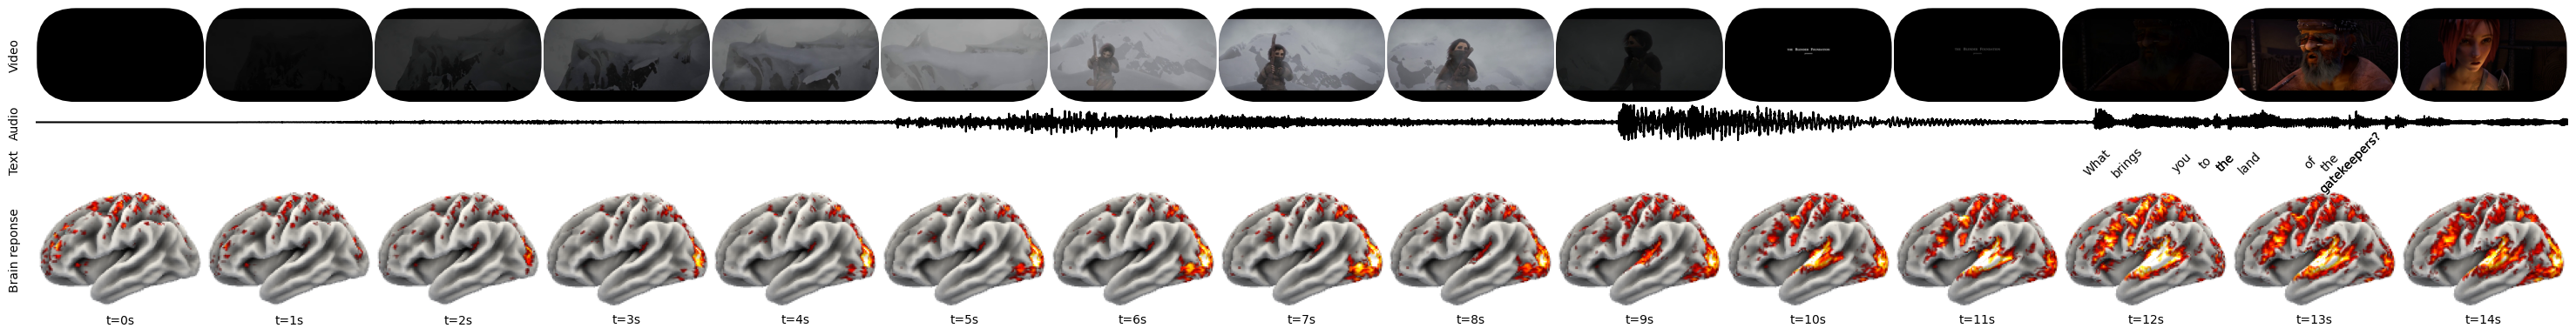
\includegraphics[width=\textwidth]{figures/fig_sintel_reference.png}
\caption{\textbf{Reference reproduction (trimodal).} Predicted cortical
activity for the first 15 TRs of the Sintel trailer. Rows: stimulus frame,
audio waveform, text (word events), and predicted activity on the lateral
surface. Word events populate the ``Text'' track at $t=12$--$14\,\mathrm{s}$;
posterior visual cortex responds to the visual stream throughout. This panel is
the pipeline control, not a study result.}
\label{fig:reference}
\end{figure}

\subsection{Application to advertisements}
Applying the (bimodal) protocol to the three advertisements produced, in every
case, activity concentrated in posterior occipital cortex that builds over the
first several seconds of continuous visual stimulation
(Figure~\ref{fig:ads}). The Surf Excel spot elicited the most sustained and
spatially extensive posterior activation across $t\approx5$--$11\,\mathrm{s}$;
the Lay's and Colgate spots showed similar but somewhat less intense posterior
responses. We describe these patterns \emph{qualitatively only}. Because the
prediction arrays were not persisted (Section~\ref{sec:deviation}) we compute no
ROI statistics and draw no comparative or affective conclusions; the ``Text''
track is empty in all three panels, a visual confirmation that the language
pathway did not contribute.

\begin{figure}[t]
\centering
\begin{tabular}{@{}c@{}}
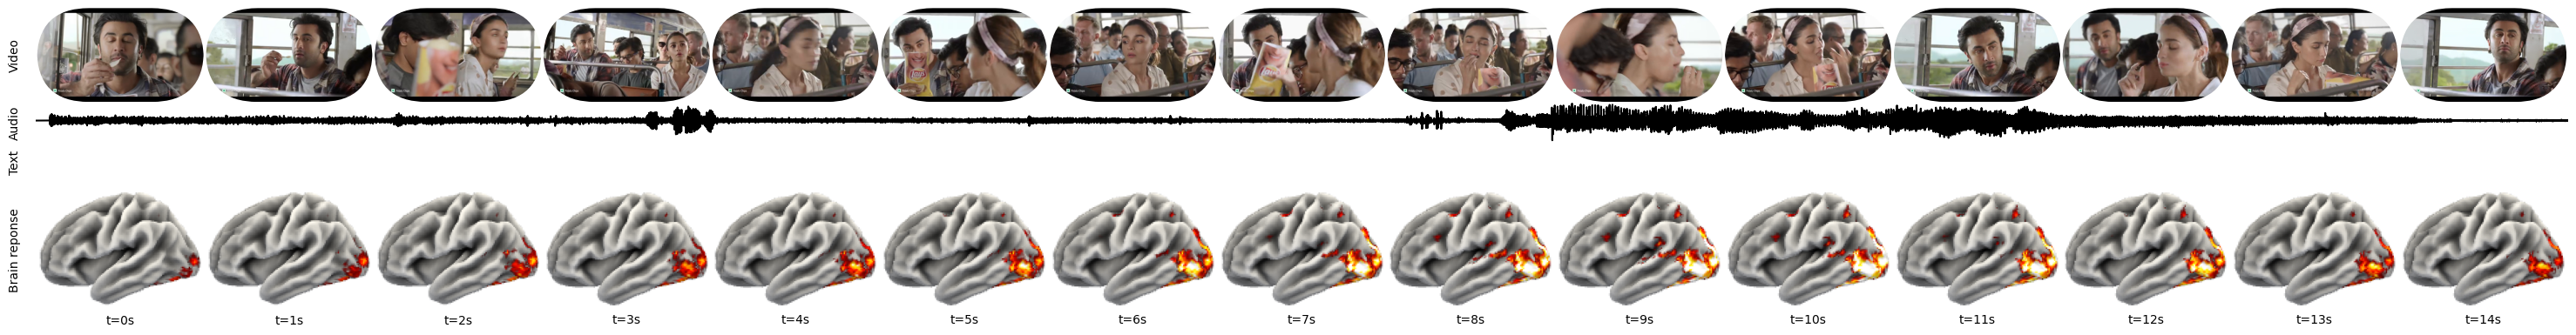
\includegraphics[width=\textwidth]{figures/fig_lays.png}\\[2pt]
{\small (a) Lay's --- ``More smiles per mile'' (25.09\,s)}\\[6pt]
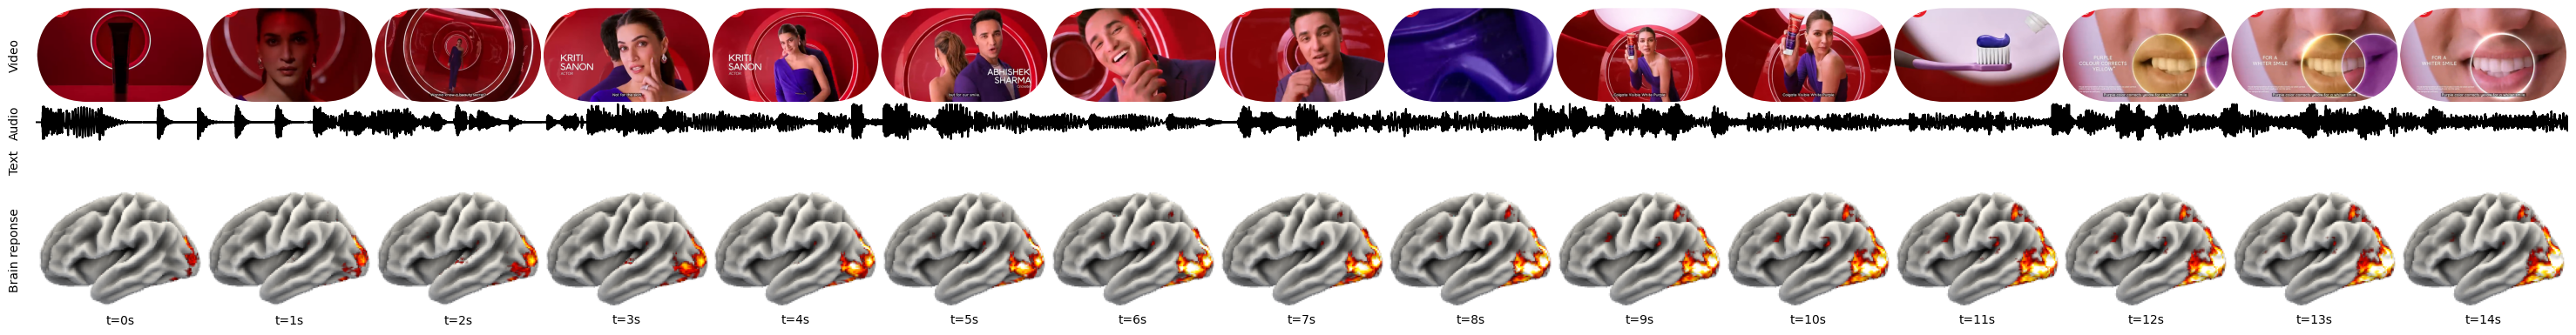
\includegraphics[width=\textwidth]{figures/fig_colgate.png}\\[2pt]
{\small (b) Colgate Visible White --- Hindi (20.13\,s)}\\[6pt]
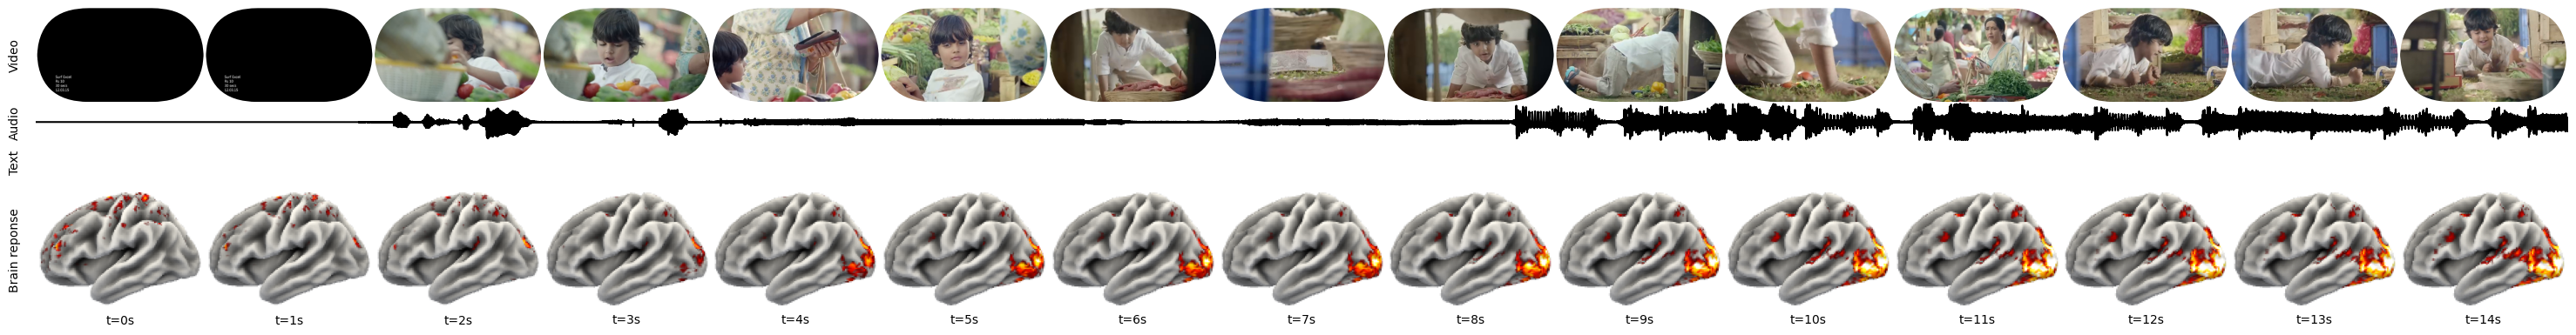
\includegraphics[width=\textwidth]{figures/fig_surfexcel.png}\\[2pt]
{\small (c) Surf Excel --- ``Primary Colours'' (33.01\,s)}
\end{tabular}
\caption{\textbf{Bimodal demonstration on three FMCG advertisements.} Predicted
cortical activity for the first 15 TRs. In all three, the ``Text'' track is
empty (word events were filtered out before prediction) and activity is
concentrated in posterior visual cortex. Panels are a feasibility
demonstration, not validated measurements.}
\label{fig:ads}
\end{figure}

\subsection{Pipeline characteristics}
Table~\ref{tab:runs} reports the runs' measured properties. Two points warrant
clarification. First, the number of predicted TRs equals the ceiling of the
clip duration in seconds (e.g.\ 26 TRs for the 25.09\,s Lay's clip): the model
prepares up to 100 candidate one-second segments and retains those fully
covered by the stimulus, so ``segments kept'' simply tracks clip length rather
than indicating discarded data. Second, video feature extraction dominates
wall-clock time (roughly \SI{16}{\second} per encoded window on a T4), so
end-to-end time scales with clip duration---about 11--18 minutes for these
20--33\,s advertisements, and ~29 minutes for the 52\,s reference clip.

\begin{table}[t]
\centering
\small
\caption{\textbf{Measured run characteristics} (from executed notebook logs).
$T$ is the number of predicted one-second TRs; encoding time is the video
feature-extraction stage on a single T4 GPU.}
\label{tab:runs}
\begin{tabular}{@{}lccccc@{}}
\toprule
Stimulus & Duration (s) & Resolution & fps & $T$ (TRs) & Video encoding \\
\midrule
Sintel (reference) & 52.21 & $854\times480$ & 24 & 53 & 29\,min 26\,s \\
Lay's              & 25.09 & $640\times360$ & 25 & 26 & 13\,min 44\,s \\
Colgate            & 20.13 & $640\times360$ & 25 & 21 & 11\,min 14\,s \\
Surf Excel         & 33.01 & $640\times360$ & 25 & 34 & 17\,min 34\,s \\
\bottomrule
\end{tabular}
\end{table}

% ============================================================================
\section{Discussion}
\label{sec:discussion}

\subsection{What the demonstration shows}
The protocol runs end to end on free cloud hardware and produces cortical
response estimates whose gross spatial structure is plausible: visual cortex
tracks the visual stream, and the trimodal reference run additionally engages
language-related cortex when speech is present. This establishes
\emph{feasibility} of scanner-free, participant-free neural response estimation
for naturalistic video---the core promise of brain-encoding foundation
models---using an entirely open toolchain that a small group can operate.

\subsection{Transferability beyond advertising}
\label{sec:transfer}
Nothing in the protocol is specific to marketing. Any short naturalistic video
can be substituted, which situates the method within the clinical and
digital-phenotyping aims of this Research Topic: standardised film clips are
already used as cognitive and affective probes \citep{hasson2004}, and a
scanner-free estimate of
the expected cortical response to such a probe could support
hypothesis generation, stimulus selection, or triage before committing scarce
imaging resources. We stress that clinical use would require the validation in
Section~\ref{sec:validation} and, ultimately, comparison against measured
neural data in the target population---neither of which we claim here.

\subsection{Limitations}
We are deliberately explicit:
\begin{itemize}[leftmargin=1.4em,itemsep=0.12em,topsep=0.2em]
  \item \textbf{No ground truth.} No EEG/fMRI or behavioural criterion was
  available, so predictive validity is untested.
  \item \textbf{Bimodal runs.} The language pathway was inactive
  (Section~\ref{sec:deviation}); results reflect video and audio only.
  \item \textbf{No persisted arrays.} Only rendered plots survive, precluding
  quantitative analysis of the existing runs.
  \item \textbf{Small stimulus set and single ``subject.''} Three
  advertisements and the model's default subject identifier do not support
  generalisation claims.
  \item \textbf{Domain shift.} TRIBE~v2 was trained on predominantly
  English-language, Western naturalistic media; applying it to Hindi-language
  Indian advertisements is an out-of-distribution use whose accuracy is
  unknown and plausibly reduced.
\end{itemize}

\subsection{Explainability, bias, and privacy}
\label{sec:ethics}
The Research Topic foregrounds explainable AI, bias, and data security, and the
method engages all three. \textbf{Interpretability:} encoding-model outputs are
spatial and temporal, hence inspectable against known functional anatomy (the
visual-cortex response is a face-valid check), but the mapping from stimulus
features to vertices remains opaque and should be probed with perturbation and
ablation analyses. \textbf{Bias:} the domain-shift limitation above is
squarely an equity issue---a model trained on Western media may estimate less
accurately for other languages and cultural contexts, and validation must be
stratified accordingly. \textbf{Privacy:} a genuine advantage of the
hardware-light approach is that inference collects \emph{no} neural or personal
data from any individual; the only human data enter through the optional,
consented self-report panel of the validation protocol, which should follow
standard ethical review.

\subsection{Conclusion}
We have presented a transparent, reproducible protocol for estimating cortical
responses to naturalistic video with an open brain-encoding foundation model,
demonstrated its feasibility on three advertisements against a reference
control, and specified the validation needed to make quantitative claims. The
value is methodological and infrastructural: an auditable, low-cost recipe that
lowers the barrier to naturalistic stimulus--response neuroscience, and a
candid map of the gap between a working pipeline and a validated measurement.

% ============================================================================
\section*{Reproducibility and data availability}
The notebooks, the figure-extraction script (\texttt{paper/extract\_figures.py}),
and the recovered figures are in the project repository:
\url{https://github.com/souricebunny/NeuroMarketing}. The model is
\texttt{facebook/tribev2} on the Hugging Face Hub. No human-participant data
were collected for this work.

\section*{Conflict of interest}
The authors declare that the research was conducted in the absence of any
commercial or financial relationships that could be construed as a potential
conflict of interest.

\section*{Author contributions}
R.G.\ designed and executed the computational pipeline, performed the analyses,
recovered and prepared the figures, and drafted the manuscript. M.K.\ supervised
the project, provided methodological guidance, and critically revised the
manuscript. Both authors approved the submitted version.

\section*{Funding}
This research received no specific grant from any funding agency in the public,
commercial, or not-for-profit sectors. % TODO(authors): confirm or add funding.

\section*{Acknowledgements}
We thank the developers of TRIBE~v2 and its constituent open models. This work
was carried out at Amity University under the supervision of Dr Misha Kakkar.

% ============================================================================
\bibliographystyle{plainnat}
\bibliography{references}

\end{document}
